\documentclass[11pt,a4paper,twoside]{book}
\usepackage[utf8]{inputenc}
\usepackage[english]{babel}
\usepackage{amsmath}
\usepackage{amsfonts}
\usepackage{pgfplots}
\usepackage{booktabs}
\usepackage{amssymb}
\usepackage{graphicx}
\author{Ege Özkan}
\title{CENG 422 \\ \large{Design and Managment of Computer Networks Lecture Notes}}
\begin{document}
\newcommand{\unsure}{\textit{?\textsuperscript{*}}}
\newcommand{\missed}{\textit{!\textsuperscript{*}}}
\maketitle
\chapter{Data and Signals - October 20, 2020}
To be transmitted, data must be transformed to electronic signals. Data can be \textit{analog} or it could be \textit{digital}.

\begin{description}
\item[Analog Data] is the information that is continious. It may have a range of infinite values. They tend to be periodic.
\item[Digital Data] is the information that has discrete states. It can only have a limited number of values. They tend to be non-periodic.
\end{description}

\section{Signal Types}

\subsection{Periodic Analog Signals}

Periodic analog signals can be classified as \textit{simple} or \textit{composite}. Two signals may have the same phase and frequency but different amplitudes. The frequency determines the amount of repeats a signal has in a time period.
\begin{figure}
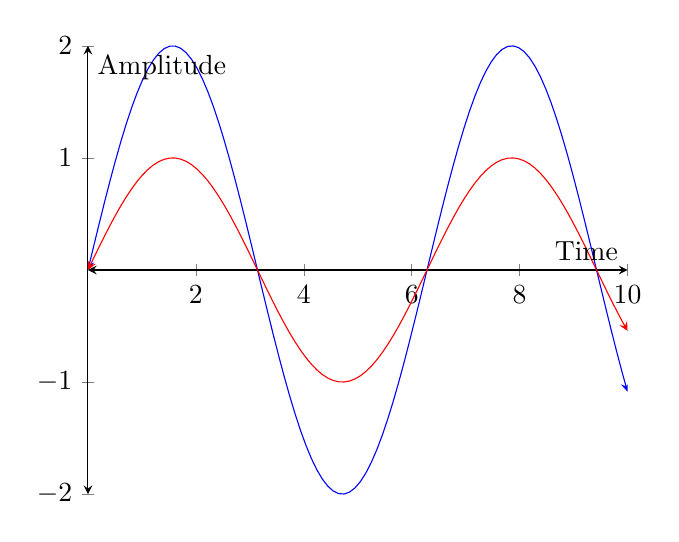
\begin{tikzpicture}[>=stealth]
    \begin{axis}[
        xmin=0,xmax=10,
        ymin=-2,ymax=2,
        axis x line=middle,
        axis y line=middle,
        axis line style=<->,
        xlabel={Time},
        ylabel={Amplitude},
        ]
        \addplot[no marks,blue,<->] expression[domain=0:10,samples=100]{2*sin(deg(x))} 
                    node[pos=0.75,anchor=south west]{};
        \addplot[no marks,red,<->] expression[domain=0:10,samples=100]{sin(deg(x))} 
                    node[pos=0.65,anchor=south west]{}; 
    \end{axis}
\end{tikzpicture}
\caption{Two waves with sample phase and frequency but different amplitude.}
\end{figure}

A period is the amount of time (in seconds) a signal needs to complete 1 cycle, given as $T = \frac{1}{f}$ where $f$ is the frequency.

\begin{figure}
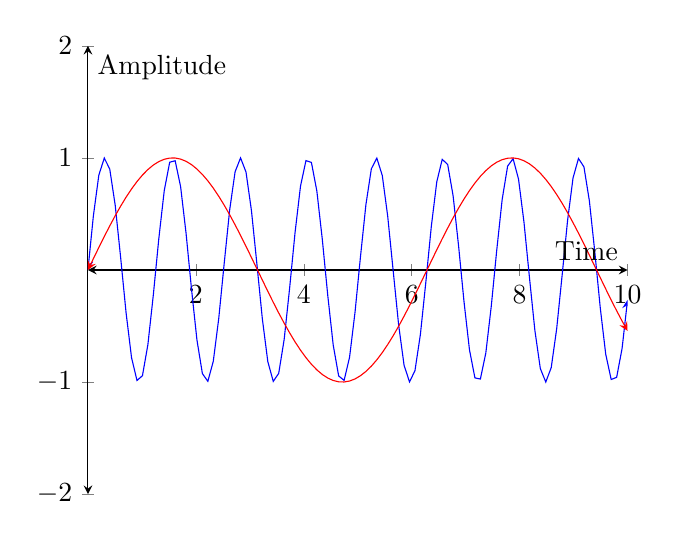
\begin{tikzpicture}[>=stealth]
    \begin{axis}[
        xmin=0,xmax=10,
        ymin=-2,ymax=2,
        axis x line=middle,
        axis y line=middle,
        axis line style=<->,
        xlabel={Time},
        ylabel={Amplitude},
        ]
        \addplot[no marks,blue,<->] expression[domain=0:10,samples=100]{sin(5*deg(x))} 
                    node[pos=0.75,anchor=south west]{};
        \addplot[no marks,red,<->] expression[domain=0:10,samples=100]{sin(deg(x))} 
                    node[pos=0.65,anchor=south west]{}; 
    \end{axis}
\end{tikzpicture}
\caption{Two waves with sample amplitude and phase but different frequency.}
\end{figure}

Frequency is the rate of change with respect to time. Change in a short span of time means high fequency. Otherwise a low frequency. If a frequency does not change at all, its frequency is zero. If the change is instantenious, it is infinite.

\begin{figure}
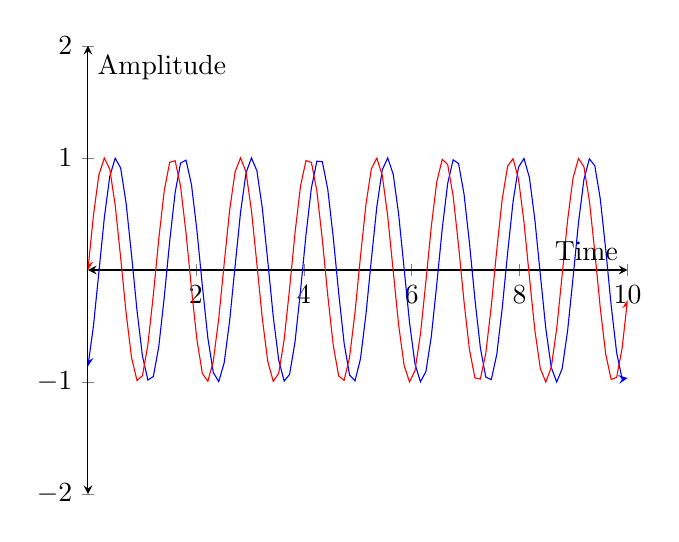
\begin{tikzpicture}[>=stealth]
    \begin{axis}[
        xmin=0,xmax=10,
        ymin=-2,ymax=2,
        axis x line=middle,
        axis y line=middle,
        axis line style=<->,
        xlabel={Time},
        ylabel={Amplitude},
        ]
        \addplot[no marks,blue,<->] expression[domain=0:10,samples=100]{sin(5*deg(x + 1.05))} 
                    node[pos=0.75,anchor=south west]{};
        \addplot[no marks,red,<->] expression[domain=0:10,samples=100]{sin(5*deg(x))} 
                    node[pos=0.65,anchor=south west]{}; 
    \end{axis}
\end{tikzpicture}
\caption{Two waves with sample amplitude and frequency but different phase.}
\end{figure}

The wavelength describes the distance a signal can travel during a period.\\

The waves may be represented using only their frequency domains, simplifying their graphs significantly.

\subsubsection{Composite Signals}

According to Fourier analysis, any composite signal consists of simpler simple signals. If the composite signal is periodic, the decomposition gives a series of signals with discrete frequencies. If the composite signal is nonperiodic, the decomposition gives a combination of sine waves with continuous frequencies.

The \textit{bandwith} of a signal is the difference between the maximum frequency and the minimum frequency it consists of.

\begin{equation}
B = f_h - f_l
\end{equation}

\subsection{Digital Signals}

In digital signals, the amplitude is divided into levels, as the number of levels increase, so does the speed of the transmittion. The \textbf{bitrate} represents the number of bits sent per second. Number of bits that can fit in a number of levels if the number of levels are $n_L$ is:

\begin{equation}
n_B = \log_2 n_L 
\end{equation}

A \textbf{bit length} is the distance that a bit occupies on the transmission medium. Tranmission speed times bitrate.

\begin{equation}
L_B = v \times r_b
\end{equation}

A periodic digital signal occupies an infinite amount of discreate freuqiencies. Whereas non-periodic digital signals (which most of them are.) occupy a continous range of infinite frequencies.\\

\textbf{Baseband transmission} is sending a digital signal through a channel without changing it to analog first.

A digital signal necessitates a low-pass channel, a channel that starts from 0Hz.\\

In general, any transmission losses \textit{some} information with regards to the wave form of the signal, to preserve the shape of the signal completely, one needs a low-pass channel with an infinite or very wide bandwith. Sometimes, the digital signal may have to be convert to correspodning analog signals to preserve information.\\

The required bitrate for a bandwith of $b$ is at minimum $\frac{b}{2}$. To acquire better result, once can multiply this number with harmonic sequences.\\

\textbf{Bandpass} is a channel with a limited range of frequencies $f_1 < f < f_2$. A digital signal cannot pass through a bandpass, as it is not a lowpass channel, therefore, the signal is first converted to analog, sent through the channel and then converted back to the digital. These include telephone lines.\\

\section{Tranmission Impairment}

\begin{description}
\item[Attenuation] is the lose of amplitue in the medium, and amplifier can be used to mitigate this issue. The lose and gain can be calculated with the dB unit.
\item[Distortion] Due to the difference of behaviour of the medium for difference frequiences, parts of the composite signal may arrive out of phase, or different.\\
\item[Noise] They may be \textbf{Thermal  Noise} due to the random motiof of electrons in the wire. \textbf{Induced Noise} is noise due to motors or appliences in the environment. \textbf{Crosstalk Noise}, effect of one wire on the other and \textbf{Impulse Noise} is a sudden spike in electricity in the wire. The quality of the medium can be calculated via the SNR (Signal-to-Noise Ratio), higher the SNR, higher the quality of the signal.
\end{description}

\section{Data Rate Limits}

A very important considiration in communication is how fast the data can be sent, in bits per second, over a channel. Keep in mind that, increasing the levels of a signal may reduce the reliability of the system.

\subsection{Formulas}

Maximum data rate of a channel for a noisless channel is the Nyquist formula $L\times n_B \times \log_2 L$ \unsure and for a noisy channel is the Shannon Formula, Capacity $=$ bandwith $+$ $\log_2(1 + \text{SNR})$

\section{Performance}

The bandwith can be calculated in hertz or in bits per second. \textbf{Bandwith delay} is the number of bits that can fit into a channel.
\missed

\chapter{Transmission Media \& Ethernet - October 27, 2020}

Different media was used in history to transfer data. From telegraph to telephone.\\

The media itself can be divided to \textit{Guided} and \textit{Unguided} transmission media. Where guided is the wired and unguided is the wireless.

\section{Guided Media}

\subsection{Twisted-pair Wire}

Consists of two cables twisted around each other. Twisted-pair cables are more resiliant against noises. As a twisted-pair of $P^+$ and $P^-$ cables are affected by the noise the same amount, hence the reciever can understand the actual signal by $(P^+ + N) - (P^- - N) = P^+ - P^-$. Cancelling noise.\\

Twisted pairs come in two variants, UTP (the unshielded pair.) and STP (the shielded pair.), UTP tends to be more widespread due to its cheapness.\\

Attenuation, the amount of information lose, tends get worse \textit{faster} the thinner it is, therefore, the loss of information is worse for thinner cables.

\subsection{Coaxial Cable}

The coaxial cable carries the ground connection as a shield, and the main signal as  the cable.

\subsection{Optical Fiber}

Optical fiber is used to refract light in its core between two cladding between a sender and a reciever. This method uses the critical angle reflection of the light. When a light is sent at a critical angle to a less dense environment from a more dense environment, it reflects.

\subsubsection{Propoagation Modes}

Light propagates in different ways inside a optical fiber, different fibers use different modes. Fiber optic cables are divided into \textbf{Multimode} and \textbf{Single mode} cables. Multi-mode cables are then divided to \textbf{Step index} and \textbf{Graded index} fiber optic cables.\\

Optical fibrer cables has a zone in its wavelength, around $1400$nm where there is high loss.\\

IN general fiber provides higher bandwith, less signal attenuation, immune to electromagnatic interference, resistance to corrosion, lightweight, greater immunity to tapping howeever, it tends to be more difficult to install and maintain, has unidirectional light propagation and it costs more.

\section{Unguided media}

Wireless communication can use between 3kHz and 900THz. Different propagation methods can be used to send data. Ground propagation, where signals below 2MHz travels paralel to the ground, following curvature. Sky propagation, where signals between 2 and 30MHz can reflect off the Ionosphere and reach. And finally, line-of-sight propagation, where, above 30MHz, signals need to have a direct line-of-sight, as they tend to pass through the ionosphere.\\

Wireless transmission can be done using radiowave, microwave and infrared.\\

Antenna's also come in two variations, \textbf{omnidirectional}, where signal travels in all directions, as well as \textbf{unidirectional}, which comes in dish and horn antenna, where waves travel in single directions.

\section{Ethernet}

Ethernet was the culmination of IEEE project 802 in 1985, to set standards to enable intercommunication between different equipment\\

Divided into two sublayers, logical link control (LLC) and Media access control (MAC).\\

Most upper layer protocols (such as IP), do not use LLC.

the standard ethernet A connectionless, unreliable service. Each frame was sent independently, when a frame is lost or corrupted, reciever drops it.

\begin{table}
\begin{tabular}{ll}
\toprule
Version & Speed \\
\midrule
Standard Ethernet & 10Mbps \\
Fast Ethernet & 100Mbps \\ 
Gigabit Ethernet & 1Gbps \\
Ten-gigabit Ethernet & 10Gpbs \\
\bottomrule
\end{tabular}
\end{table}

Ethernet consists of a preamble, 56 bits of alternating 1s and 0s. SFD, the start frame delimiter (10101011), destination adress, source adress, length or type and data and padding, following that, a CRC.\\

Ethernet used to use Carrier sense multiple access with collision detection, called CSMA/CD. That is, the sender listens to the cable to detect collusion, in which case it waits for a while and resends the frame.\\

Data and padding portion of the data must be at least 46 bytes, and at most 1500 bytes. The existence of the minimum length arose from the fact that at least 46 bytes was necessary for CSMA/CD to work.\\

An example ethernet adress in hexademical looks like $7a:79:19:92:d8:98$. The adresses are divdied into unicast and multicast adresses, where the lest significant bit of the first byte is 0 for unicast adresses, and 1 for multicast addresses.\\

The broadcast destination address is a special case of the multicast adress in which all bits are 1s. This adress are used to send to the DHCP server to retrieve information.\\

Standadr ethernet has different implementations, 10Base5, 10Base2, 10Base-T and 10Base-F.

In the standard ethernet, Manchester Encoding/Manchester Decoding was used. Where the transformations between 0 and 1 signals in data was themselves encoded using 1s and 0s.

The second revision of the ethernet removed the CSMA/CD, data transfer became bidriectional, moved all computers to their own domain, and introduced Fast Ethernet, which did not support bus topology. It was implemented into three forms. Manchester was also discarded due to it needing too much bandwith.\\

The third revision introduced the Gigabit ethernet, MAC layer was changed to the full-duplex version. It had four implementations.\\

The tenth gigabit ethernet is possible only with fiber-optic technology. Supporting LAN PHTY and WAN PHY, working in full-duplex.

\chapter{Bandwith Utilization - November 10, 2020}

Bandwith utilization is different method of manuplating bandwith in order to decrease cost, increase privacy, or add noise tolarance.

\section{Multiplexing}

Whenever the bandwith of a medium linking two devices is greater than bandwith needed by both, the link can be shared by multiple connections \unsure. This process is called \textit{Multiplexing} with Multiplexers used to multiplex multiple signals and Demultiplexers (Demux) being used to convert them back to single signals.

\subsection{Frequency Divison Multiplexing}

An \textit{analog} method of multiplexing is used when different baseband analog signals are recieved. They are moudlated with different modulator signals, and are summed together, being sent through the medium.\\

In the demultiplexing step, filters are used to distinguish signals, and then each signal is put through a demodulator, recieving the original signals.\\

In FDM, guard bands might be used as buffer zones between different channels to avoid channels from generating parasite.\\

Different ways of encoding signals may also be used in FDM, such as QAM, which uses phase shifting.\\

Multiple FDM multiplexers may be bound in chains, generating groups, supergroups, master groups and jumpgroups and so on. This methods are [or were] conventionally used in telephone systems. This is called an \textit{analog hierarchy}.

\subsection{Wavelength Division Multiplexing}

Another \textit{analog} system, used in finer cables which use light; WDM may use prism as multiplexers and demultiplexers.

\subsection{Time Division Multiplexing}

A \textit{digal} method, TDM allocates time slots to each device, and uses buffers to accumalate data in between sending.

\subsection{Synchronous TDM}

Synchronous TDM sends frames, each frame subdivided to its own subdivisions. \unsure.

Synchronization must be achieved to make sure data being sent is recieved correctly. Sometimes, this issue is resolved via the introduction of a \textbf{framing bits}, additional bits added to the start of frames, adhering to a agreed upon synchronization pattern.\\

In sTDM, empty slots may occur, since data of each device is sent at the same time, sometimes a device may not send data at that time, its slots is left empty.\\

Likewise with analog methods, TDMs may also be chained together. creating a \textit{digital hierarchy}.

Since analog signals can be converted to digital signals, telephone lines and other analog systems can also be used with TDM after conversion. [And, in fact, nowadays, most telephone systems have become digital.]

\subsection{Statistical TDM}

By introducing additonal information before data, the occurance of empty slots may be removed.

\section{Spread Spectrum}

In spread spectrum, signals from different sources are combined to fit into larger bandwith, this may be to prevent eavesdropping, jamming, or to increase noice tolarance.\\
\begin{description}
\item[Frequency Hopping Spread Spectrum (FHSS)] The original signal is spread using a frequency table, that generates frequencies using a synthezier depending on the data origniating from a pseudo-random code generator, this frequency is combined with the original signal using a modulator. FHSS results data \textit{hopping} between frequiencies, increasing noise tolarance and also making eavesdropping harder.
\item[Direct-Sequence Spread Spectrum (DSSS)] adds predefined data to the original data, making it harder for the signal to be understood by anyone who does not know about the predefined data.
\end{description}

\chapter{Wireless LANs: WiFi \& Bluetooth - November 10, 2020}

\section{WiFi}

Defined by IEEE 802.11 specification as a Basic Service Set (BSS) or an Extended Service Set (ESS).

\subsection{Service Sets}

A BSS without an Access Point (AP), a dedicated device like a router,  is called an \textit{ad hoc network}. A BSS with an AP is called an \textit{infrastructure network}.\\


An Extended Service Set occurs when multiple Access Points are connected thorugh a distribution system, and is controlled by a server or a gateway. It should be noted that a device might be connected to multiple BSSs simultaniously in an ESS.\\

\subsection{Physical Layer}

IEEE 802.11 consists of a physical layer which support many different protocols, and a data link layer consisting of a MAC sublayer and \missed.\\

Different protocols may use different modulations.

\subsection{Data Layer}

A variation of CSMA/CA (\S 2.3) that uses signals such as CTS (Continue to Send), RTS (Request to Send), ACK (Acknowledgment), as this process continues between a source and destination; at the same time, all other stations not partaking in this data transfer, stop transferring data, this is called NAV, since signals carry with them the time it will take for data transfer, they do not even listen to the conversation, avoiding noise. This entire process is called \textbf{DCF} [Distributed Coordination Function].\\

An alternative to DCF is called \textbf{PCF} (Point coordination Function). Here, the Access Point asks each station if it has any data to send (called \textbf{polling}), this occurs one-by-one. This process occurs in a round-robbin style, and this time is called a \textbf{contention-free}. Since PCF must be backwards compatible, there is also a contention zone following each contention-free zone, where stations that do not support PCF can contact the AP in a DCF fashion.\\

[I just want to say the term robbin is also used when describing some chess tournaments.]\\

\subsection{Frame Format}

Frame format of WiFi contains four different addresses to define a data transfer. Depending on the value of the To DS and From DS flags, different addresses contain different data, for instance, if both flags are set to 1, addresses are used for sending AP, recieving AP, source station and destination station respectivelly.\\

\subsection{Frequencies}

WiFi uses three frequency bands chiefly, around 900MHz, around 2.4GHz and around 5.8 GHz. Different frequency bands are also subdivided into different channels. The

\subsection{Problems}
Wifi has its unique problems due to its wireless nature, where ranges of devices may cause significant issues.

\subsubsection{Hidden Station Problem}

Station A is inside the range of both C and B, but C and B cannot see each other, this causes CSMA/CA to function incorrectly, introducing problems.\\

This is solved by the fact that the RTS signal of the WiFi contains the time it will take for data to transfer, since CTS signal from A also contains this time data, this functions as a form of \textit{handshaking}, where when a station realises a CTS signal isn't sent to itself, it goes into NAV.\\

\subsubsection{Exposed Station Problem}

Occurs when A-B and C-D pairs are trying to send data to each other, but A and C can hear each other, when D and B cannot, causing either A or B to go into NAV unnecasserily.

\section{Bluetooth}

A bluetooth network is called a \textbf{Piconet}, the device the bluetooth originates from is called a \textbf{primary}, whereas devices connected to it is called a \textbf{secondary}. A secondary on a piconet may become a primary for another piconet, creating a \textbf{scatternet}.\\

\textbf{Logical Link Control and Adaption Protocol (L2CAP)} is used for data exchange on an ACL link. It is equivalent to an LLC layer of ethernet, whereas the \textbf{Baseband Layer} corresponds to the MAC layer of LAN, it uses Time Division Multiplexing.\\

Communication in a piconet is handled in a round robin fashion, whereas a time slot is used to send data, another to recieve data, and repeat until all secondaries have been given permission recieve and asked to send data.


\chapter{Frame Relay \& ATM - November 17, 2020}

Frame Relay is a virtual-circuit wide-area network that was designed in response to demands for a new type of WAN in the late 1980s and early 1990s.

\section{Point to Point Circuit}

Dedication of a physical line between two routers. This method, although straightforward and simple, is high-cost, and not suitable for burst data. (Tranmission of large amounts of data).

\section{Frame Relay}

The frame relay was created as a response to these complaints, where multiple routers are connected to a single source, the Frame Relay, and the frame relay directs the packages to their destinations.\\

Frame Relays consists of virtual circuits called DLCIs, Data Link Connection Identifier. They consists of two layers, Phyiscal and Data Link layers, Physical layers support ANSI standards, and the Data Link layer consists of simplified core functions.\\

A frame layer frame consists of a flag, an adress, information, FCS and a flag. The address section consists of 6 bits of DLCI, 1 bit for Command response, 1 bit for extended adress flag, 4 bits of DLCI, 1 bit FECN, 1 bit of BECN, 1 bit DE, 1 bit of Extended Adress flag. FECN and BECN holds information about congestion in the network. the DE Flag notifies if the package is eligible for discarding if congestion occurs.\\

Frame Relay does not contain error control. These must be provided in upper layers.\\

DLCI addresses may be two, three or four bits lengths.\\

FRADs can bridge between Frame Relays and diffferent types of networks.

Frame Relay has a problem with Multiplexing, simce the frames are big, small packages are congested by a channel sending big packages.

\section{ATM}

Asynchronous Transfer Mode is the cell relay protocol designed by the ATM forum and adopted by the ITU-T.\\

ATM was designed to make sure hardware handles as much of the communication as possible.\\

ATM solves the problem with multiplexing frames using \textbf{cell}s, cells are small units of information, keeping congestion to a minimum.\\

ATM multiplexing also do not use the round robin system that causes empty package slots, instead the ATMs header has enough information on it that the switches know where the packages are going.\\

Much like the Frame Relay, ATM uses virtual connections, going through Virtual paths, going through virtual transmission paths.\\

A virtual connection is defined by a pair of numbers, the VPI (Virtual Path Identifier) and the VCI (Virtual Circuit Identifier).\\

UNI connections that occur between users and the switches has less space for VPI (16 bits VCI to 8 bits VPI) compared to NNI connections, which occur between netowrks (16 bits VCI to 12 bits VPI).\\

ATM consists of three layers, a Physical an ATM and finally a AAL (Application Adaptation Layer). Originally, the physical layer for ATM was SONET, a fiber-optic network standard designed to transfer large amount of data.\\

ATM provides routing, traffic managment and multiplexing.\\

In the UNI cells, there is an extra ATM header for GFC (Generic Flow Control) stealing space from VPI. otherwise, both cell structures consists of PT, CLP and HEC fields in the header.

\subsubsection{AAL connections}

\begin{description}
\item[AAL1] Supports continous data transmission.
\item[AAL2] Packages of changing data size.
\item[AAL3/4] Connection orianted services.
\item[AAL5] Simple but large volumes of data. (Simple but Effective Layer)
\end{description}

In today's world, AAL1 (for Streaming Audio and Video) and AAL5 (for data communications) is used.\\

\subsubsection{ATM LANs}

ATM is mainly a Wide-Area network protocole (WAN ATM) but it is also possible to use ATM in LAN.

\begin{figure}[httb]
\centering
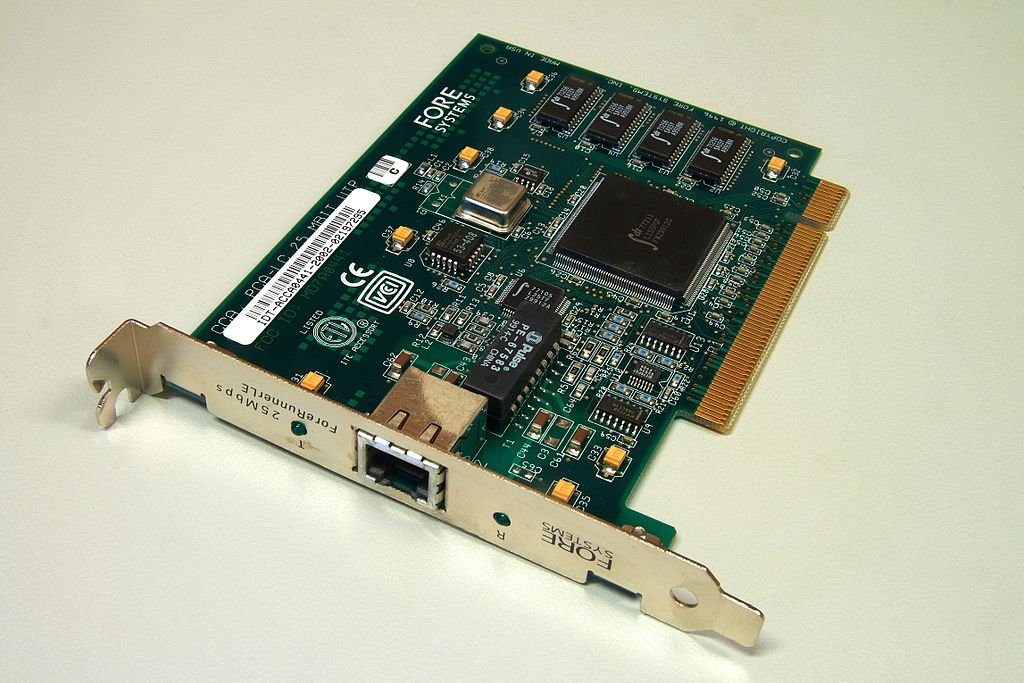
\includegraphics{atmcard.jpeg}
\caption{FORE Systems ForeRunnerLE 25 ATM Lan Card by Wikipedia user Barcex}
\end{figure}

Computers that will connect to the ATM LANs (without converters) will need a dedicated network card, just like an Ethernet Card. ATM LANs are not used widespread.

\chapter{Logical Addressing - November 17, 2020}

A logical address is an adress that stays the same. Physical adresses, in the meantime, changes while going from network to network.

\section{IPv4 Adresses}

An IPv4 address is a \textbf{32-bit} address that uniquely and universally defines the connection of a device (a computer, a computer, or a router) to the internet.

\begin{enumerate}
\item They are unique and universal.
\item They are 32-bits long.
\item The address space of IPv4 is $2^{32}$.
\end{enumerate}

It can be written in Dotted-decimal notation, such as 128.11.3.31 With each part being between 0 and 255.\\

\subsection{Classful Adressing}

In classful addresing, there are five classes of IP addresses. Each IP address consists of two parts, Network ID (netid) and Host ID. netid stays the same for an organization :(is the ID of the entire organization) Hostid, in the meanwhile, is a single machine at that organization.\\

Depending on the class (A, B, C) the size of the netid/hostid changes.

\begin{table}
\begin{tabular}{lll}
\toprule
& Network ID & Host ID \\
\midrule
Class A & 1 &  2, 3, 4\\
Class B & 1, 2 & 3, 4 \\ 
Class C & 1, 2, 3 & 4 \\
Class D/E & -- & -- \\
\bottomrule
\end{tabular}
\end{table}

In Class A the first, the class B the second, and in the class C first three bits are specific.

\begin{table}
\begin{tabular}{llll}
\toprule
& Block Count & Block Size & Application \\
\midrule
Class A & 128 &  16,777,216\\
Class B & 16,384 &  65,536 \\ 
Class C & 2,097,152 & 256 \\
Class D & 1 &  2,147,483,648 & Multicast\\
Class E & 1 & 2,147,483,648 & Reserved\\
\bottomrule
\end{tabular}
\end{table}

\subsubsection{Mask}

\begin{table}
\begin{tabular}{lll}
\toprule
& Dotted-Decimal & CIDR \\
\midrule
Class A & 255.0.0.0  & /8\\
Class B & 255.255.0.0 & /16 \\ 
Class C & 255.255.255.0& /24 \\
\bottomrule
\end{tabular}
\caption{The default masks for classful addressing}
\end{table}

The mask is a special bit sequence that, when logical anded with an IP address, returns the netid, this way, we can determine where to send the packages.

\subsection{Classless Addressing}

Classful addressing has become obsolete, due to many problems in its, namely, too many adresses going to waste. Nowadays, ISPs tend to grant a \textbf{block} of addresses is given to a user.\\

Here the mask is written in CIDR to the end of the address, for instance \texttt{x.x.x.x/n} where \texttt{n} is the address mask. A block of this calibre starts with \texttt{x.x.x.x}s last \texttt{n} bits zeroed and continues to \texttt{x.x.x.x} with its last bits oned. Moreover, this block containts $2^{32 - n}$ adresses. Routers do this by ANDing with the mask for finding the first address and ORing with the mask's complement for finding the last, they add one to the Mask's complement to find the number of addresses.\\

Adress blocks are granted containing addresses of powers of two.\\

\subsection{The Network Adress}

The first address in a block is normally not assigned to any device. It is used as the network adress. It represents the network as a whole.

\subsection{Subnets}

Subnets are used to divide up the IP to different sized ranges. For instance, an IP network of 17.12.14.0/26 can be divided into a range of /27 and two ranges of /28.

\chapter{Logical Addressing (Cont`d) - November 24, 2020}

\section{NATs}

Since there is a limited number of IP addresses, Local IP ranges are provided in the standard. Within a network, a NAT router (or software) swaps the headers of incoming and outgoing packages accordingly.\\

NAT routes give private ports to the internal local IP addresses.\\

\newcommand{\C}[1]{\texttt{#1}}

\begin{table}
\begin{tabular}{lll}
\toprule
Start & End & Size \\
\midrule
\C{10.0.0.0} A & \C{10.255.255.255}  & 24 Bits \\
\C{172.16.0.0} & \C{172.31.255.255}& 20 Bits \\ 
\C{192.168.0.0} & 192.168.255.255 & 16 Bits \\
\bottomrule
\end{tabular}
\caption{Local Ranges}
\end{table}

The NAT system can also be used by ISPs to serve more IPs.

\section{IPv6}

IPv6 is 128-bit addressing system that is the new standard, still not accepted by many ISPs, it was created in response to the shrinking pool of IPv4 addresses. They are originally writting in Hexadecimal, such as \C{FDEC:0074:0000:0000:0000:B0FF:0000:FFF0}, abbreviated as \C{FDEC:74:0:0:0:B0FF:0:FFF0}, or in the most abbreviated form \C{FDEC:74::B0FF:0:FFF0}.\\
 
IPv6 has type prefixes at the start, they denote different sorts of networks.

\begin{table}
\begin{tabular}{ll}
\toprule
& Type\\
\midrule
\C{010} & Provider-Based Unicast Address\\
\C{100} & Geographic-based Unicast Addresses\\
\C{1111 1110 11} & Site Local \\
\C{1111 1110 10} & Link Local \\ 
\bottomrule
\end{tabular}
\caption{IPv6 prefixes}
\end{table}

Here the provider based unicast addresses are addresses given to a provider, geographic based unicast addresses are ones given to geographic entities, Site Local and Link Local can be given to companies. Multicast addresses are given to a group of computers.\\

\subsection{Reserved Addresses}


\begin{table}[httb]
\begin{tabular}{ll}
\toprule
Description & Fraction \\
\midrule
All zeros & Unspecified, used by computers unaware of their IP addresses.\\
Last bit 1, otherwise zero & Loopback\\
Compatible and Mapped & Used for transition from IPv4 \\
\bottomrule
\end{tabular}
\caption{Reserved Addresses}
\end{table}

\chapter{Network Layer: Internet Protocol - November 24, 2020}

When sending a package locally, within the same network, the data link layer is sufficient to send the data between computers.\\

But once we need to send data between routers, bigger networks, we need to add a network layer on top of the Data Link layer. Network Layer is able to find the Host-to-Host path.\\

In the earlier days of the internet, networks were unable to talk with each other. Even today, certain protocols such as SMP only works in the data link layer.\\

The network layer contains a routing table to understand where to send and how to send data.

\begin{figure}[httb]
\centering
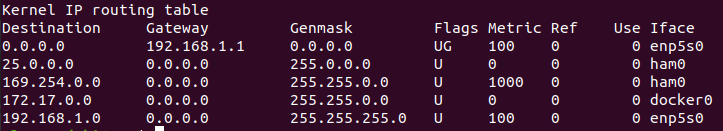
\includegraphics[scale=0.5]{routingtable.png}
\caption{A Routing Table at a computer}
\end{figure}

Communication at the network layer in the internet is connectionless, that is, data is send before establishing a connection.

\section{IPv4}

IPv4 is the format used in the network layer, its packages are called \textbf{datagram}s with an adjustable header length, Service bits (which denote the sevice), a field denoting the protocol, and many other fields, and of course, most importantly, source and destination IP.\\

IPv4 also includes a \textit{time to live} field, that denotes how many hops will go before a router discards a package, used to stop loops from occurring. It also includes a checksum for the header.

The IPv4's header is between 20 to 60 bytes. While the whole package can be $2^{16} - 1$ bytes long.\\

The service type also includes a precedence field to denote the precedence of the package, this was never used in practice, however.

\begin{table}
\begin{tabular}{ll}
\toprule
& Type\\
\midrule
\C{0000} & Normal\\
\C{0001} & Minimize cost\\
\C{0010} & Maximize reliability \\
\C{0100} & Maximize throughput \\
\C{1000} & Minimize delay\\ 
\bottomrule
\end{tabular}
\caption{IPv4 Service Field Values \& Meanings}
\end{table}

Certain services \textit{require} certain service field values.\\

When sending a small datagram in an ethernet frame, we may have to pad it, since a minimal package is 20 bytes long while ethernet requires a bigger package for minimum.

MTU, the Maximum Transfer Unit, is used to denote the largest transferable package side for a network. According to the MTU value, package might be fragmented, however, the Do Not Fragment flag might be set in the datagram to denote to the network \textbf{not} to fragment a package, in which case the package will be dropped, and the sender will be notified. The fragment offset flag may be set to denote which fragment this is, or how many more fragments there is, etc. etc.

There are some other options here, one can set which routers will be used for instance.

\section{IPv6}

IPv6 born as the IPv4 pool shrinked, the IPv6 has a bigger header field, space for extensions, resource allocation, authentication and encryption.\\

Because the first 40 bytes are always the same, the devices working with IPv6 datagrams have easier time compared to IPv4.\\

IPv6 added priorites for congestion controlled traffic. If the traffic gets congested, depending on the priority of the traffic. If the source can adapt itself to the traffic, it is called congestion-controlled traffic, if not it is called noncongestion-controlled, congestion-controlled traffic goes from 0 to 7, and noncongestion goes from 8 to 15, higher the number, more prioritised should be the package.

\section{Transition from IPv4 to IPv6}

\begin{description}
\item[Dual Stack] Systems that support IPv4 and IPv6 simultaneously.
\item[Tunnelling Strategy] IPv6 host \textit{tunnels through} the IPv4 region, the IPv6 datagram is embed inside the IPv4 datagram.
\item[Header Transition] an IPv6 package's headers can be modified into an IPv4 package if the IPv6 source wants to reach an IPv4 region.
\end{description}


\chapter{Process-to-Process Delivery - December 1, 2020}

Most prominent process-to-process delivery protocols are UDP and TCP, with a newly emerging protocol of SCTP.\\

The transport layer is responsible for Process to Process delivery, delivery of a packet, part of a message, from one process to another. Two processes communicate in a client/server relationship.\\

Process to Process is the third main type of delivery covered in this course, Node to Node (Data link layer), Host to Host (Network layer), and now, Process to Process.

\section{Client-Server Model}

The server program has a dedicated port on its host computer. The client, on the other hand, may be assigned a random port, called a \textbf{Ephemeral Port}.

\section{IANA}

IANA assigns port numbers to new applications, the ranges are defined as follows:

\begin{table}
\begin{tabular}{lll}
\toprule
& Name & Explanation \\
\midrule
0-1023 & Well-Known & Registered and controlled by IANA. \\
1024-49,151 & Registered & Registered but not controlled by IANA. \\ 
49,152 - 65,535 & Dynamic & Ephemeral ports independent from IANA. \\
\bottomrule
\end{tabular}
\end{table}

\section{Socket Address}

Socket address is the combined IP and port number

\section{Features of Transport Control}

Transport control allows demuxing and muxing.\\

\subsubsection{Connectionless Service}

A connectionless service is created when a package is sent without controlling if the destination is open or not. (Without a connection being established.)

\subsubsection{Error Control}

There is no error control between transport, network and datalink layers. (In general).

\section{Protocols of the Transport Layer}

Running on top of the IP protocol. There are three.

\subsection{User Datagram Protocol (UDP)}

The user datagram has a simple package format, being independent of each other, the header is eight bytes long, with two bytes each for a source port number, destination port number, total length and checksum, followed by the actual data payload.\\

UDP package length is equal to the data length of the IP package it is sent in.\\

UDP Packages form queues in both the receiver and transmitter end. Flow control and error control is not provided by UDP, custom software must be used to provide these features.

\subsection{Transport Control Protocol (TCP)}

TCP is by far the most popular transfer protocol. It uses \textit{stream delivery}, just like writing to a file. It is also a connection aware service.\\

Buffers are sometimes used between bytes, data that is sent but not confirmed to be received may stay around or a while, to send it again.\\

\subsubsection{TCP Segments}

TCP packages are send as segments, they provide flow control and error control. Segments are enumerated by TCP, the numbering starts with a randomly generated number. (This enhances security)

A segment's header consists of a 16 bits of each source and destination port address, 32 bits each sequence number and acknowledgment number, acknowledgment number defines the byte number receiver is expecting to receive.\\

The header further has six flags in the control field. These control the state of the connection. \\

\begin{table}
\begin{tabular}{ll}
\toprule
Name & Explanation \\
\midrule
SYN & Synchronise sequence numbers.\\
FIN & Close connection.\\
RST & Reset the connection.\\
PSH & Pushes the data without a package is filled.\\
ACK & Denotes that a package is an acknowledgment.\\
URG & Denotes that the package is urgent, prioritise in queue.\\
\bottomrule
\end{tabular}
\end{table}

Denial of Service (DOS) attacks are done by trying to establish many SYN connections on a target server.\\

TCP uses a three-way handshaking to establish connection.\\

Half-close refers to when a side closes down its TCP connection prior to the other side.

\subsubsection{Sliding Window}

Sliding windows refers to the number of packages a TCP connection will last if no acknowledgment is send from the other size. Window size is calculated by the minimum of receiver and network congestion.

\subsection{Stream Control Transmission Protocol (SCTP)}

SCTP allows for multiple streams of data to be opened between two processes. These streams are called \textit{association}s.\\

SCTP supports multihoming, allows for multiple IP addresses to be used for receiving and sending data.\\

Data chunks are identified by three items: TSN, SI and SSN.\\

SCTP uses four-way handshaking, which mitigates DOS attacks.

\chapter{Domain Name Service - December 8, 2020}

DNS, or Domain Name Server is a special server that converts between domain namse and domain IPs.

\section{Name Space}

Either Flat or Hierarchical, IP addresses are bound to the names. Generally used Hierarchically, the names are defined in an inverted tree with dots separating them.\\

FQDN is the full address, PQDN is the Partial address, where the rest of the address is completed according to the network configuration.\\

Consider that hierarchical name spaces allows for multiple servers hierarchically pointing to each other. The global Root servers hold the address for the TLD domain servers like \C{.com}, \C{.edu}.\\

A primary server loads all information from the disk file, the secondary server loads all information from the primary server.\\

There are different domain types, Generic Domains (TLDs), country domains (ccTLD), Inverse domains, etc.\\

There are two types of records, queried using UDP 53 protocol. Unless if the result is too big, in that case the TCP 53 is used.\\

Registrars are commercial entities accredited by ICANN to register new DNS records.\\

Dynamic Domain Name System (DDNS) can be used to update the DNS automatically.


\chapter{Remote Logging, Mail Servers - December 15, 2020}

\section{TELNET}

\textbf{Remote Logging} refers to using another computer as your own, (logging into a computer). \textbf{TELNET} can be used to logging into any computer's any port. TELNET can only be used with TCP.\\

In contemporary usage, TELNET has been replaced in many usages by other, more secure, technologies such as SSH, SSH can be used with encryption.\\

\subsubsection{NVT Character Set}

A special character set, called the NVT character set is used to convert characters automatically to make sure different sorts of computers can speak to each other.\\

The First bit of the NVT character determines if the character is a control character (1) or normal (0). The control characters carry commands.\\

Four special characters are also used for negotiation \C{WILL}, \C{WONT}, \C{DO}, \C{DONT} is used to determine which parts of the connection will be handled by the host versus the server.

\section{Electronic Mail}

E-Mail can work in  very different ways. Even without internet if both users are on the same computer, then, we only need two \textbf{User Agent}s. But if the traffic is over the internet, then we need two \textbf{Message Transfer Agent}s to facilitate  the trade of emails. Two UAs and two MTAs (one server, one client).\\

In the more complicated variation, there may be a \textbf{mail server}, a dedicated machine for the receiving and sending of emails.\\

The fourth and final variation of email transfer occurs with two computers connecting over two dedicated mail servers, the receiving end of it stores the messages until the receiver connects with an MAA client, and thus contains an MAA server. The MAA is used to receive messages.\\

The action of sending a mail is called \textbf{pushing} messages. The action of getting messages from MAA server is called \textbf{pulling}.\\

Examples of command-driven user agents are \C{mail}, \C{pine} and \C{elm}. On the other hand, GUI-based user agents are Outlook and Thunderbird.

\subsubsection{The Nature of Email}

An email consists of an \textbf{envelope} and \textbf{message}. The envelope consists of the addresses messages arrives from and goes to. \textbf{RFC 821} defines the envelope standard, \textbf{RFC 822} defines the message standard.\\

An Email address has the structure \C{local@domain}, where \C{local} is the name of the local address of the user in the mail server at \C{domain} address.

\subsubsection{MIME}

MIME is the translation layer between 7-bit NVT ASCII codes and Non-ASCII codes.\\

The MIME headers in the E-Mail Header section of the E-Mail message hold information about the message in the email body.

\subsection{SMTP}

the \textbf{Simple Mail Transfer Protocol} is used to transfer mail from the sender client to the receiver mail server. Defined in RFC 821, SMTP is used between the sender client and the sender client and the sender server and the receiving client \textit{but not} between the receiving server and the receiving client.\\

The SMTP commands follow the format \C{command:keyword}. Port 25 is used for SMTP in the TCP.

\subsection{POP3 \& IMAP4}

The \textbf{Post Office Protocole} (POP3) and \textbf{Internet Mail Access Protocol} (IMAP4) is used in the receiving end of the connection. Between the receiving client and the server holding the emails of the receiver.\\

The greatest distinction between IMAP4 and POP3 is that, with POP3, the mail is stored in the recipient computer, and is deleted from the server. In IMAP4, the mails are stored in the server.

\section{File Transfer}

Transferring files from one computer to another is generally done through \textbf{File Transfer Protocol} (FTP).\\

FTP uses to TCP connections simultaneously, Port 20 and 21. The port 21 is used for sending commands (control connection) and 20 is used for data transfer. This way, commands can still be send during download.\\

The Control Connection of the FTP uses NVT. The data connection's file type, data structure and transmission mode are defined by the client. The text mode is used to convert line ending between Unix and Windows (\C{CRLF} vs \C{LF}).

\chapter{DHCP - December 15, 2020}

\textbf{Dynamic Host Configuration Protocol} is responsible for assigning information to hosts. The DHCP arose from \textbf{BOOTP}, (and is backwards compatible with it).

\section{BOOTP}

BOOTP is a protocol used to ask for the IP Addresss, gateway information etc. As well as extra information such as where the operating system of the computer is. It uses port 67.\\

\section{DHCP}

DHCP is built on BOOTP. It provides the address, subnet mask, gateway, name server and many other information to the connecting computers.\\

DHCP has a pool of available addresses that it can assign to hosts as they need, these addresses last for a \textit{lease time} and expires after this, though the host may renew it.

\chapter{SNMP - January 5, 2020}

SNMP is a simple network management protocol.

\end{document}
